\section{Modeled Circuits}
\label{sec:modeled-circuits}
    \frame{\sectionpage}

    \begin{frame}
        \frametitle{Choice criteria}

        \begin{itemize}
            \item Not too simple, not too complex
            \item Familiar to any hardware designer
                \begin{itemize}
                    \item No signal processing, etc.
                \end{itemize}
            \item Well-defined, language-agnostic specification
                \begin{itemize}
                    \item Results to validate the models against
                \end{itemize}
        \end{itemize}

        \note{
            \begin{itemize}
                \item Too simple: tutorials, every EDSL would shine
                \item Too complex: too much effort in design, too little in analysis
                \item Language-agnostic: Not base the correctness in an EDSL version
            \end{itemize}
        }
    \end{frame}

    \begin{frame}
        \frametitle{Chosen circuits}

        \par{We cherry-picked circuits from the book ``Elements of Computing Systems'',
            as they satisfied all of our demands.}

        \begin{figure}[h!]
            \includegraphics[width=0.5\textwidth]{imgs/book-cover-elements.jpg}
            \caption{``Elements of Computing Systems'' - Nisan, Schocken, \newline
                available at \url{http://www.nand2tetris.org}.
                \label{fig:book-cover-elements}
            }
        \end{figure}
    \end{frame}

    \begin{frame}
        \frametitle{Chosen circuits}

        \begin{description}
            \item[Circuit 1] A 2-input, 16-bit-wide, simple ALU
            \item[Circuit 2] A 64-word long, 16-bit wide memory bank
            \item[Circuit 3] An \emph{extremely} reduced instruction set CPU,
                the \emph{Hack} CPU.
        \end{description}
        \vspace{0.05\textwidth}

        \par{Let's take a quick look at each of these circuit's specification\ldots}
    \end{frame}


    \subsection{ALU}
    \label{subsec:alu}
        \begin{frame}
            \frametitle{Circuit 1: ALU}

            \par{Some of the circuit's key characteristics:}

            \begin{itemize}
                \item 2 \emph{operand inputs} and 1 \emph{operand output}, each 16-bit wide
                \item 1 \emph{output flag}
                \item Can execute 18 different \emph{functions}, among which:
                    \begin{itemize}
                        \item Addition, subtraction
                        \item Bitwise AND / OR
                        \item Constant outputs
                        \item Increment / decrement
                        \item Sign inversion
                    \end{itemize}
            \end{itemize}

            \note{
                \begin{itemize}
                    \item Operands in two's complement notation
                \end{itemize}
            }
        \end{frame}

        \begin{frame}
            \frametitle{Circuit 1: block diagram}

            \begin{figure}[h!]
                \centerline{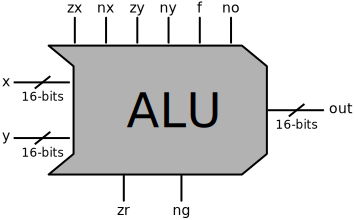
\includegraphics[width=0.6\textwidth]{imgs/alu-block.pdf}}
                \caption{Input/Output ports of \emph{circuit 1}, the ALU.
                    \label{fig:alu-block}}
            \end{figure}

            \note{
                \begin{itemize}
                    \item Operands -- control -- flags
                \end{itemize}
            }
        \end{frame}

        \begin{frame}
            \frametitle{Circuit 1: specification}

            \par{The behaviour of the ALU is specified by the values of the \emph{control bits} and \emph{flags}:}

            \begin{description}
                \item[\texttt{zx} and \texttt{zy}]
                    \emph{Zeroes} the ``\texttt{x}'' and ``\texttt{y}'' inputs, respectively
                \item[\texttt{nx} and \texttt{ny}]
                    \emph{bitwise negation} on the ``\texttt{x}'' and ``\texttt{y}'' inputs
                \item[\texttt{f}]
                    Selects the function to be applied: \newline
                    $\text{``\texttt{f}''} = 1$ for addition, $\text{``\texttt{f}''} = 0$ for bitwise AND
                \item[\texttt{no}]
                    \emph{bitwise negation} on the output ALU output
                \item[\texttt{zr} and \texttt{ng}]
                    The output \emph{flag} $\text{``\texttt{zr}''} = 1$ \emph{iff} the ALU output is zero.
                    $\text{``\texttt{ng}''} = 1$ \emph{iff} the output is negative.
            \end{description}

            \vspace{0.3cm}
            \par{Formal definition and test cases in the book.}

            \note{
                \begin{itemize}
                    \item Specification: rules defining output/flags in terms of the inputs/ctrl
                \end{itemize}
            }
        \end{frame}


    \subsection{Memory bank}
    \label{subsec:memory-bank}
        \begin{frame}
            \frametitle{Circuit 2: RAM64}

            \par{Some of the circuit's key characteristics:}

            \begin{itemize}
                \item \emph{Sequential} circuit, with clock input
                \item 64 memory words stored, each 16-bit wide
                \item Address port has width $\log_{2} 64 = 6$ bit
            \end{itemize}

            \note{
                \begin{itemize}
                    \item Clock input not present in the models (implicit)
                \end{itemize}
            }
        \end{frame}

        \begin{frame}
            \frametitle{Circuit 2: block diagram}

            \begin{figure}[h!]
                \centerline{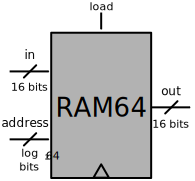
\includegraphics[width=0.45\textwidth]{imgs/ram-block.pdf}}
                \caption{Input/Output ports of \emph{circuit 2}, the RAM64 block.
                    \label{fig:ram-block}}
            \end{figure}
        \end{frame}

        \begin{frame}
            \frametitle{Circuit 2: specification}

            \begin{itemize}
                \item The output ``\texttt{out}'' holds the value at the memory line indicated by ``\texttt{address}''.
                \item \emph{Iff} $\text{``\texttt{load}''} = 1$,
                    then the value at input ``\texttt{in}'' will be loaded into memory line ``\texttt{address}''.
                \item The loaded value will be emitted on ``\texttt{out}'' at the \emph{next} clock cycle.
            \end{itemize}

            \note{
                \begin{itemize}
                    \item Starting value not mentioned in the spec. Chose zero
                \end{itemize}
            }
        \end{frame}


    \subsection{CPU}
    \label{subsec:cpu}
        \begin{frame}
            \frametitle{Circuit 3: Hack CPU}

            \begin{itemize}
                \item A \emph{very} reduced instruction set CPU
                    \begin{itemize}
                        \item Only 2 instructions: ``\texttt{C}'' and ``\texttt{A}''
                    \end{itemize}
                \item Follows the \emph{Harvard architecture}
                    \begin{itemize}
                        \item Separate \emph{data} and \emph{instruction} memory blocks
                    \end{itemize}
                \item Instructions are 16-bits wide
                    \begin{itemize}
                        \item As well as the memory input and output
                    \end{itemize}
                \item Two \emph{internal} registers: ``\texttt{D}'' and ``\texttt{A}''
            \end{itemize}
        \end{frame}

        \begin{frame}
            \frametitle{Circuit 3: block diagram}

            \begin{figure}[h!]
                \centerline{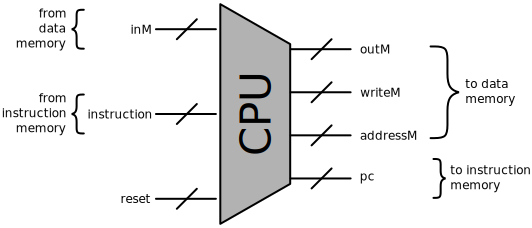
\includegraphics[width=1.0\textwidth]{imgs/cpu-block.pdf}}
                \caption{Input/Output ports of \emph{circuit 3}, the \emph{Hack} CPU.
                    \label{fig:cpu-block}}
            \end{figure}
        \end{frame}

        \begin{frame}
            \frametitle{Circuit 3: specification}

            \par{Circuit 3 runs ``\texttt{A}'' and ``\texttt{C}'' instructions, according to the \emph{Hack assembly specification}.}
            \vspace{0.3cm}

            \begin{itemize}
                \item The ``\texttt{A}'' instruction: sets the ``\texttt{A}'' register.
                    
\includegraphics[width=0.8\textwidth]{imgs/cpu-instruction-a.pdf}
                \vspace{0.5cm}
                \item The value in ``\texttt{A}'' can be used:
                    \begin{itemize}
                        \item As operand for a subsequent computation
                        \item As address for jumps
                    \end{itemize}
            \end{itemize}

            \note{
                \begin{itemize}
                    \item 1-bit instruction code
                \end{itemize}
            }
        \end{frame}

        \begin{frame}
            \frametitle{Circuit 3: specification}

            \par{Circuit 3 runs ``\texttt{A}'' and ``\texttt{C}'' instructions, according to the \emph{Hack assembly specification}.}
            \vspace{0.3cm}

            \begin{itemize}
                \item The ``\texttt{C}'' instruction:
                    sets the ``\texttt{C}'' register, performs \emph{computation} or jumps.
                    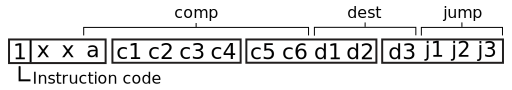
\includegraphics[width=0.85\textwidth]{imgs/cpu-instruction-c.pdf}
                \vspace{0.5cm}
                \item Some peculiarities:
                    \begin{itemize}
                        \item Bits ``\texttt{c1}'' to ``\texttt{c6}'' control the ALU
                        \item \emph{conditional} or \emph{unconditional} jumps
                        \item \emph{destination} of the computation result: ``\texttt{A}'', ``\texttt{D}'', ``\texttt{M}''
                    \end{itemize}
            \end{itemize}
        \end{frame}

        \begin{frame}
            \frametitle{Circuit 3: specification (parts)}

            \begin{figure}[h!]
                \centerline{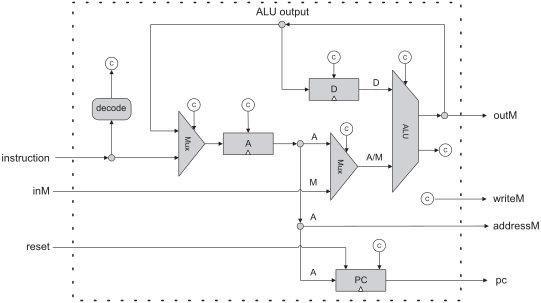
\includegraphics[width=1.05\textwidth]{imgs/cpu-parts.pdf}}
                \caption{Parts used to build the \emph{Hack} CPU, and their interconnection.
                    \label{fig:cpu-parts}}
            \end{figure}
        \end{frame}
